
\documentclass[a4paper,11pt]{article}
% define the title
\usepackage{graphicx}
\author{GDP Group18}
\title{UAV Image Viewer User Guide}
\begin{document}
% generates the title
\maketitle
%\newpage
% insert the table of contents
%\tableofcontents
%\newpage
\section{Things to do Before Starting the UAV Image Viewer Program}
In order to connect the payload and camera with the UAV,
the user need an ethernet cable to plug in the back of the UAV controller,
and another end to the payload controller.
The payload controller power, send and receive command form this ethernet cable.
The user do not have to connect the camera manually as it is already connected.
If the user want to disconnect and reconnect the camera using a new wire, 
the user can refer to the schematic diagram.
On the ground side, the UAV data receiver connect to the computer by connect one end which is USB printer cable to the receiver, and the USB side to the computer.
Figure~\ref{clipArt} shows the diagram of how to connect the payload to the UAV and the UAV data receiver to the computer. 

\begin{figure}[!htbp]
\begin{center}
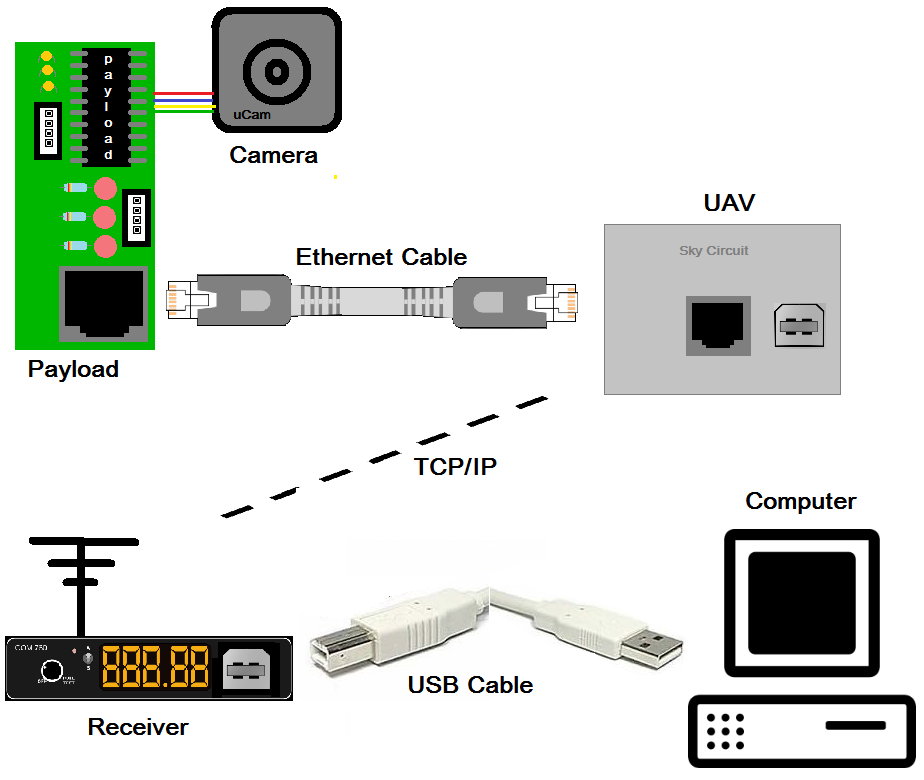
\includegraphics[scale=0.4]{clipArt.png} 
\caption{The Clip Art of the Hardware Connection Diagram\label{clipArt}}
\end{center}
\end{figure}

To make the UAV Image Viewer work correctly, the ground station must be connect to the receiver first. 
In order to connect to the receiver, all the hardware have to connect as described in section1.
The GCS station then connect to the Autopilot receiver by clicking on the Connect button. If the program does not connect to the Autopilot automatically , the user can choose it from the combo box. Then tick the box to Enable Network Server. Figure\ref{GCS} shows a screen shot of the GCS program
If the autopilot does not appear, the user should check the connection of the UAV and make sure that the driver of the USB has already installed. 

To install the USB driver:

 run the device manager $\rightarrow$ right click on the UAV $\rightarrow$ click on the update driver$\rightarrow$ find the driver $\rightarrow$ install it $\rightarrow$ UAV is ready to use.

\begin{figure}[!htbp]
\begin{center}
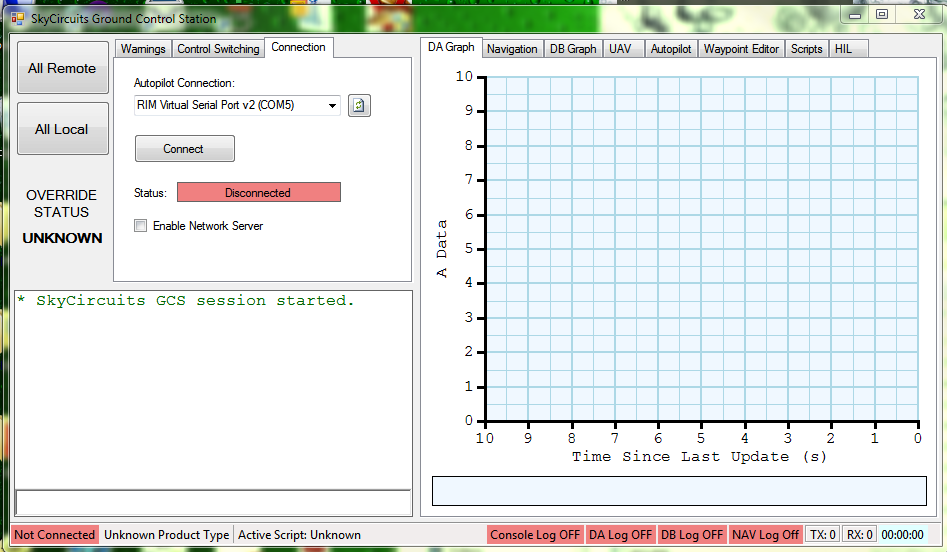
\includegraphics[scale=0.5]{GCS.PNG}  
\caption{The Ground Control Station Software\label{GCS}}
\end{center}
\end{figure}
 


\section{UAV Image Viewer Ground Station}

\begin{figure}[!htbp]
\begin{center}
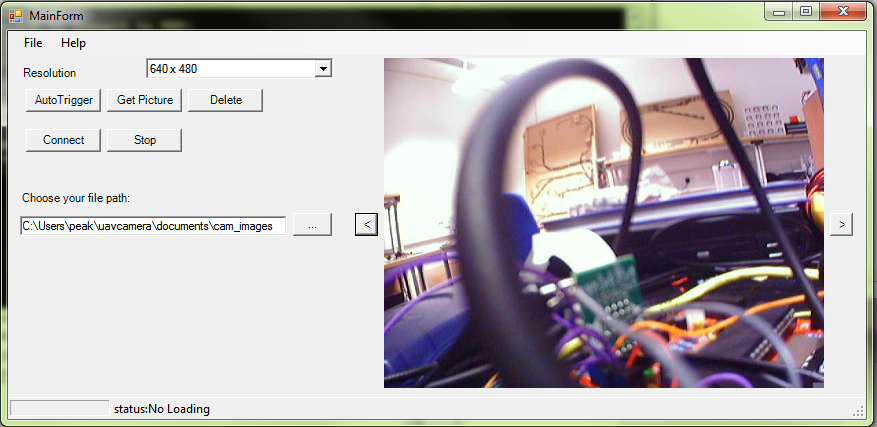
\includegraphics[scale=0.6]{windowApplication.PNG}  
\caption{The UAV Image Viewer Software\label{IVP}}
\end{center}
\end{figure}

The file tab on the top left corner allow the user to open a file to display it onto the picture box or save the image that is displaying on the picture box to a specified directory. It also give the option to exit the program. Figure\ref{openTab} shows the diagram of the file tab.

\begin{figure}[!htbp]
\begin{center}
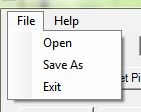
\includegraphics[scale=1]{FileButton.png}  
\caption{Open Tab\label{openTab}}
\end{center}
\end{figure}

The user can choose the resolution from the program in the top left. There are four options of the resolution that the camera can take, The lower the resolution the faster the downloads of the image. 

\begin{figure}[!htbp]
\begin{center}
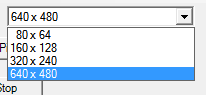
\includegraphics[scale=1]{comboBoxResolution.png}   
\caption{The Resolution Option\label{resOp}}
\end{center}
\end{figure}

In figure\ref{buttons} shows buttons of the program applications. The Auto trigger button allows the user to take multiple photo and save it on board on the SD card. The Get Picture button will allow the user to take the picture and send the picture to ground station. The picture file name will be uavPictureAtyyyy-MM-dd\_hh-mm-ss-tt.jpg. The photo will be saved in the specified file path in the text box as shown in figure \ref{filePath}. The name depend on the date and time at the time of taking picture. It will take about 10-20 seconds to display the image. It depends on how complicate the photo is. 

\begin{figure}[!htbp]
\begin{center}
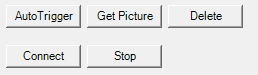
\includegraphics[scale=1]{button.PNG}  
\caption{The Buttons Options of the Image Picture Viewer\label{buttons}}
\end{center}
\end{figure}

\begin{figure}[!htbp]
\begin{center}
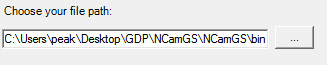
\includegraphics[scale=1]{filePath.PNG} 
\caption{The file path text box\label{filePath}}
\end{center}
\end{figure}

The left and right button near the picture allow the user to change the displaying photo to any jpeg photo in the same directory. The button has shown in figure\ref{leftRight}. 

\begin{figure}[!htbp]
\begin{center}
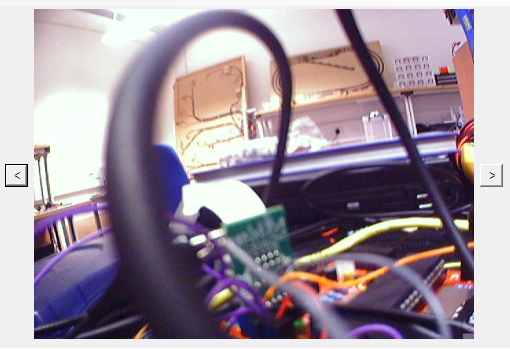
\includegraphics[scale=1]{leftRight.PNG}   
\caption{The Picture Box with left and right buttons\label{leftRight}}
\end{center}
\end{figure}

The progress bar show how much percentage have the photo arrive to the ground station. The status label will tell what signal is send and receiving so the user can keep track of what is going on inside the program.

\begin{figure}[!htbp]
\begin{center}

\includegraphics[scale=1]{progress_bar.PNG} 
\caption{The progrss bar and the status text\label{progressBar}}
\end{center}
\end{figure}

\subsection*{Take Picture}

The use can simply click on Get Picture button on the program. Figure\ref{buttons} shows where the button is.

\end{document}